% -*- root: ../thesis.tex -*-
%%%%%%%%%%%%%%%%%%%%----------%%%%%%%%%%%%%%%%%%%%
%%%
% 	Author: Boris Kourtoukov
%   Project: Digital Futures Thesis Document
%   Title: Periphery
% 	File: Narrative
%%%
%%%%%%%%%%%%--------------------------%%%%%%%%%%%%

\mqp{What comprises Periphery?}
Through the work on this project Periphery has been distilled into three clear parts: 

\begin{itemize}
  \item Stable and wearable ambient sensor network.
  \item Application Porogramming Interface (API) for the collected data.
  \item Visual style guide for future wearables.
\end{itemize}

\newthought{This chapter will} focus on the visual style guide. It was created with the support from Chenthooran Nambiarooran\sidenote{\url{http://chenthooran.com/}}, he is concept artist and illustrator based out of London.

\section{Design Inspiration}

\mqp{What influenced the development of the style guide?}
The primary inspiration for the art exploration in the project was cyberpunk literature, film, and games. Authors like William Gibson\sidenote{\url{http://www.williamgibsonbooks.com/}} and Neal Stephenson\sidenote{\url{http://www.nealstephenson.com/}} created a very intriguing depictions of what the technology of our near future would be like. Films include Johnny Mnemonic\sidenote{\url{http://www.imdb.com/title/tt0113481/}} and Blade Runner\sidenote{\url{http://bladerunnerthemovie.warnerbros.com/}} and provided a deeper visual exploration of what has become a very iconic style. While Deus Ex\sidenote{\url{http://www.deusex.com/}} explored the minutiae of this setting in much greater quantities through the need of a vast variety of in-game assets. The main problem that arises from this media is the focus on the violent uses of technology. This creates a mixture of pleasing aesthetics with a clear threatening tone. The Periphery style guide strives to focus entirely on the pleasing aspects of this media, and forgo the harsher elements.
\FloatBarrier

\section{Design Constraints and Visual Reference}\label{sec:designconstraints}

It is important to keep in mind that this is a modern day device. Although the aesthetics are deeply rooted in a great deal of our current Sci-Fi and Cyberpunk art the final outcome needs to function outdoors today.

The major environmental constraints are:

\begin{itemize}
  \item Public transit
  \item Restaurants
  \item Rain
  \item Running
  \item Bumping into things
  \item Coming into physical contact with others
\end{itemize}

\begin{marginfigure}
  \includegraphics[width=1in]{neck_modules_1.jpg}
  \caption{Early selection of modules designed to go on the neck.}
  \label{fig:neckmodules}
\end{marginfigure}

To elaborate, if the user ends up hugging someone it should not end in blood. If they trip there should not be chunks of plastic everywhere. Although the latter is largely up to the chosen materials, it has been an important influence on these concept stages.

\newthought{These concepts} provides a reference for:

\begin{itemize}
  \item Textures and patterns
  \item Key shapes
  \item The colour scheme
  \item Repeaters and Rhythm
  \item Placement
\end{itemize}

\mqt{What is the goal of the style guide?}
\newthought{The concepts that follow} is not intended as a literal blueprint. Instead, they represent various stages of thought reflecting the iterative design process that is informing the nature of these devices, and should be remixed as needed.

As mentioned, a great deal of artwork that exists today within the Cyberpunk genre is of military, violent or menacing nature it has been one of the challenges in this project to extract the aspects that make that art inspiring while detaching these negative connotations.

Prior to entering this stage the main, or summarized, constraint was that:

\begin{quote}
The outcome should be a visually inspiring, modular and practical (but only to the extent of not constricting movement and damaging innocent bystanders) set of wearables on the body.
\end{quote}

\newpage

\section{The Concepts}\label{sec:concepts}

\begin{figure}
  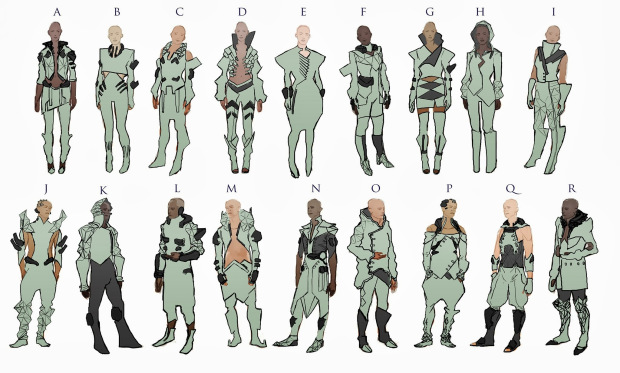
\includegraphics{clotherie1.jpg}
  \caption{Results from the second round and a set of more dynamic poses. A piece from the preliminary sketches below.}
  \label{fig:secondround}
\end{figure}

\begin{marginfigure}
  \includegraphics[scale=0.5]{figure3.png}
  %\caption{Part of preliminary sketches.}
  \label{fig:secondround}
\end{marginfigure}

Following the constraints and inspiration mentioned above, Chenthooran created a number of iterations that reflected in a final set of modules. The positions of modules were not determined from the start, although they were influenced by the ``Design for Wearability'' paper \citep{Gemperle98} described earlier. The final modules settled on the upper arms, hip, and neck. During this phase, the design has been intentionally left without the influence of physical electronic restrictions, thus allowing for a more reusable final style guide.

\begin{figure}
  \includegraphics[scale=0.5]{other_poses.jpg}
  \caption{More dynamic poses.}
  \label{fig:dynamicposes}
\end{figure}

\begin{figure}
  \includegraphics{modules1.jpg}
  \caption{Closer subset of modules.}
  \label{fig:subsetofmods}
\end{figure}

\begin{figure}
  \includegraphics{modules2v2.jpg}
  \caption{Three selected module shapes.}
  \label{fig:selectedmods}
\end{figure}

\begin{figure*}
  \includegraphics{modules3fixed2.jpg}
  \caption{A closer detail of the final shapes.}
  \label{fig:finalmods}
\end{figure*}
